\begin{frame}
\frametitle{MSAA: Demo}
\begin{figure}[ht]
    \centering
    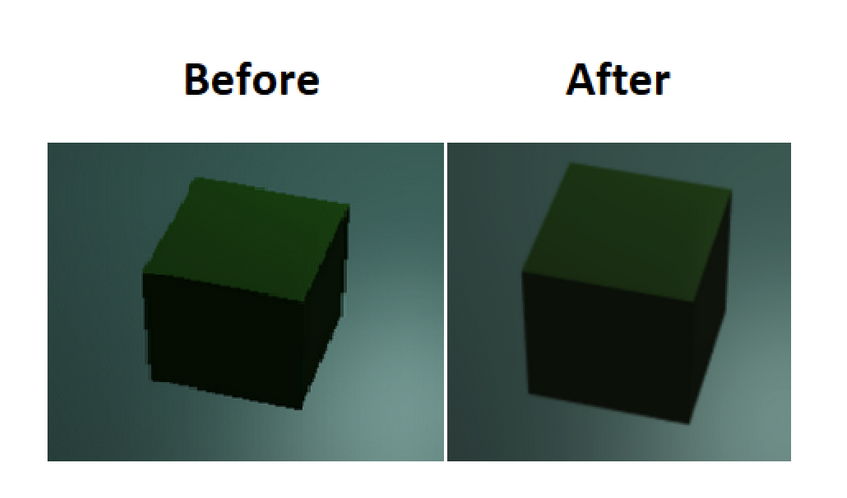
\includegraphics[scale=0.50]{images/SlidesMSAA/BeforeAfterMSAA.png}
\end{figure}
\end{frame}

\begin{frame}
\frametitle{MSAA}
\begin{itemize}
\item MSAA stà per multi sample anti aliasing
\item Abilitiamo MSAA quando creiamo il pipeline state object
\item Dobbiamo creare delle immagini che abbiano più di un campione per pixel
\end{itemize}
\end{frame}
